\documentclass[conference]{IEEEtran}
\IEEEoverridecommandlockouts
% The preceding line is only needed to identify funding in the first footnote. If that is unneeded, please comment it out.
\usepackage{cite}
\usepackage{amsmath,amssymb,amsfonts}
\usepackage{algorithmic}
\usepackage{graphicx}
\usepackage{textcomp}
\usepackage{xcolor}

\usepackage{listings}
\usepackage{color}
\usepackage{stfloats}
\usepackage{subfigure}

\definecolor{dkgreen}{rgb}{0,0.6,0}
\definecolor{gray}{rgb}{0.5,0.5,0.5}
\definecolor{mauve}{rgb}{0.58,0,0.82}

\lstset{frame=tb,
  language=Python,
  aboveskip=3mm,
  belowskip=3mm,
  showstringspaces=false,
  columns=flexible,
  basicstyle={\small\ttfamily},
  numbers=none,
  numberstyle=\tiny\color{gray},
  keywordstyle=\color{blue},
  commentstyle=\color{dkgreen},
  stringstyle=\color{mauve},
  breaklines=true,
  tabsize=3
}

\def\BibTeX{{\rm B\kern-.05em{\sc i\kern-.025em b}\kern-.08em
    T\kern-.1667em\lower.7ex\hbox{E}\kern-.125emX}}
\begin{document}


\title{Project A:Visual Interpretation of Convolutional Neural Networks}

\begin{abstract}
This paper is a report for Project A of ECE1512 2022W, University of Toronto. In the paper, we described four assigned tasks with detail, including CNN construction and training, statistic assessment, XAI based interpretation and Quantitative evaluation. For the attribution methods, we choose Grad-CAM, Grad-CAM++ and Ablation-CAM as a group of two, and we reviewed their paper and implemented corresponding functions. Moreover, we tried to analyze the performance of the XAI methods based on quantitative evaluation and gave our explanations towards the experiment.
\end{abstract}

\section{Task 1: 1-Dimensional digit classification}
\subsection{Question 1}
\begin{lstlisting}
    weight_decay = 5e-4
    model = Sequential()
    #Your code starts from here 
    model.add(Input(shape=(40,1)))
    model.add(Conv1D(25, kernel_size=5, padding='same', activation='relu', kernel_regularizer=regularizers.l2(weight_decay)))
    model.add(Conv1D(25, kernel_size=3, padding='same', activation='relu', kernel_regularizer=regularizers.l2(weight_decay)))
    model.add(Conv1D(25, kernel_size=3, padding='same', activation='relu', kernel_regularizer=regularizers.l2(weight_decay)))

    model.add(Flatten())
    model.add(Dense(10, activation='softmax', kernel_initializer=keras.initializers.RandomNormal(mean=0.0, stddev=0.5),
                    bias_initializer=keras.initializers.Zeros(), kernel_regularizer=regularizers.l2(weight_decay)))

    model.summary()
\end{lstlisting}
In this question, we build a ConvNet. It includes three convolutional layer, one flatten layer and one dense layer.
The network is listed as Fig. 1:
\begin{figure}[h] 
    \centering %图片居中
    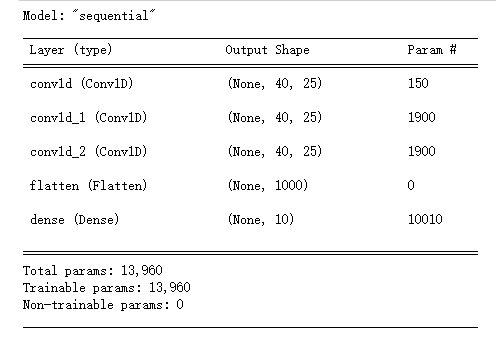
\includegraphics[width=0.3\textwidth]{T1Q1.png} %插入图片,[]中设置图片大小,{}中是图片文件名
    \caption{Task1-Question1: ConvNet Model} %最终文档中希望显示的图片标题
    \label{Fig.t1q1} %用于文内引用的标签
\end{figure}
\subsection{Question 2}
In this section, we apply the model in question 1 to the MNIST1D dataset. The code is listed as followed:
\begin{lstlisting}
    model.compile(loss=keras.losses.categorical_crossentropy,
              optimizer=tensorflow.keras.optimizers.SGD(),
              metrics=['accuracy'])

    def lr_scheduler(epoch):
        base_ep = 15
        return 1e-3 * (.5 ** (epoch // base_ep))
    lr_reduce_cb = keras.callbacks.LearningRateScheduler(lr_scheduler)
    tensorboard_cb = keras.callbacks.TensorBoard(log_dir='log2', write_graph=True)
    early_stopping_cb = keras.callbacks.EarlyStopping(patience=8, min_delta=0.)

    # X = tensorflow.expand_dims(dataset['x'],axis=2)
    train_x=dataset['x']
    train_y=dataset['y']
    train_x=train_x.reshape(4000,40,1)
    train_y=tensorflow.keras.utils.to_categorical(train_y, num_classes=10)

    # print(X.shape)
    history=model.fit(x=train_x,y=train_y,epochs=200,
    #                     steps_per_epoch=len(X) // 32,
                        callbacks=[tensorboard_cb],                  
                        shuffle = True,
                        verbose=1)
    model.save('MNIST1D.h5')
\end{lstlisting}
Here, we use the tensorboard to record the training procedure.First of all, we compile this model, set the loss function to cross-entropy, set the optimizer to Stochastic Gradient Descent and the metrics to accuracy. 
Then we define the LearningRateScheduler, the TensorBoard, the EarlyStopping for later use.
After that, we handle the train data for training.
At last, we will fit the data and tensorboard into the model for training and save the model into disk.
The training result is shown as followed\ref{Fig.t1q2}:
\begin{figure}[h] 
    \centering %图片居中
    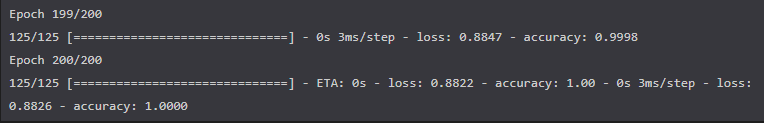
\includegraphics[width=0.5\textwidth]{T1Q2.png} %插入图片,[]中设置图片大小,{}中是图片文件名
    \caption{Task1-Question2: Training Process Log} %最终文档中希望显示的图片标题
    \label{Fig.t1q2} %用于文内引用的标签
\end{figure}
\subsection{Question 3}
\subsubsection{SubQuestion a}
TODOOOOOOOOOO, say something here.
\begin{lstlisting}
    train_acc = history.history['accuracy']
    train_loss = history.history['loss']
    plt.plot(train_acc)
    plt.figure()
    plt.plot(train_loss)
\end{lstlisting}
This is the code for loss and accuracy curve, the plot of loss curve\ref{Fig.t1q3a1} and plot for accuracy curve\ref{Fig.t1q3a2} are shown below:
\begin{figure}[h] 
    \centering %图片居中
    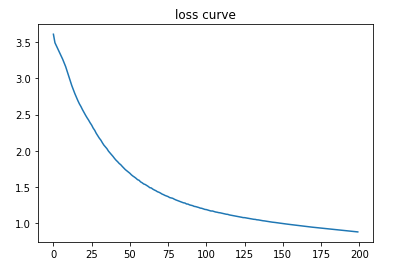
\includegraphics[width=0.3\textwidth]{T1Q3-b.png} %插入图片,[]中设置图片大小,{}中是图片文件名
    \caption{Task1-Question3a-1: Loss Curve of 1-D CNN} %最终文档中希望显示的图片标题
    \label{Fig.t1q3a1} %用于文内引用的标签
\end{figure}
\begin{figure}[h] 
    \centering %图片居中
    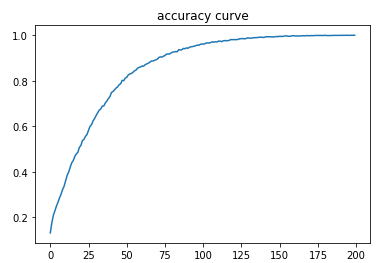
\includegraphics[width=0.3\textwidth]{T1Q3-a.png} %插入图片,[]中设置图片大小,{}中是图片文件名
    \caption{Task1-Question3a-2: Accuracy Curve of 1-D CNN} %最终文档中希望显示的图片标题
    \label{Fig.t1q3a2} %用于文内引用的标签
\end{figure}
\subsubsection{SubQuestion b}
This part talks about overall classification accuracy on the test set.

overall accuracy、 
\subsubsection{SubQuestion c}
class-wise accuracy
\subsubsection{SubQuestion d}
roc auc曲线
\subsubsection{SubQuestion e}
混淆矩阵
\subsubsection{SubQuestion f}
召回率,准确率和F-1得分

\subsection{Question 4}
挑几个正确与错误的例子,评价一下,哪两个类错误最多
\section{Task 2: CNN interprectation}


This section introduces our interpretation of 1-D CNN model based on MNIST-1D dataset using 3 different attribution methods, including our literature review, discussion and implementation of the XAI attribute algorithms.

\subsection{Grad-CAM}

\subsection{Grad-CAM++}

\subsection{Ablation-CAM}

The Ablation-CAM creatively uses ablation analysis to determine the importance of individual feature map units for different classes. It proposes a novel “gradient-free” visualization approach which avoids use of gradients and at the same time, produce high quality class-discriminative localization maps.\par

The core algorithm of Ablation-CAM is not complex: it uses the value of slope to describe the effect of ablation of individual unit $k$ by the following formula:

$$slope = \frac{y^c-y^c_k}{||A_k||}$$

In the formula, $y^c$ stands for activation score of class c, which represent the entire class activation status. $y^c_k$ indicates the value of the function for absence of unit $k$, where $A_k$ is the baseline. Those concepts lead us to ablation study, which is the basic principle of the method.\par
Ablation study is a method to distribute the influencing importance of different factors by controlling the variable while switching the combination of potential factors, and also their standalone. For example, if we'd like to know whether $A$ or $B$ component of medicine could improve the effect of an old medicine $C$. We could compare $C+A$, $C+B$ and also $C+A+B$ with the baseline of $C$. We could know if the A or B or they together are able to improve the effect. In the instance of Ablation-CAM, different unit $k$ is the "component", and the whole feature map is so-called baseline, $A_k$. Thus, using slope described in the previous formula could represent the importance of a single unit to the feature map.\par
However practically, norm $||A_k||$ is hard to compute due to its large size and hence the slope could be approximately presented by the following formula, assuming a very small value.

$$w^c_k = \frac{y^c-y^c_k}{y^c}$$

As the algorithm, Ablation-CAM can then be obtained as weighted linear combination of activation maps and corresponding weights from the formula above, which is somehow similar to that of Grad-CAM.

$$L^C_{Ablation-CAM}=ReLU(\sum_k {w^c_k}{A_k})$$

There are a number of advantages and features of Ablation-CAM. Firstly, a significant contribution and novelty of the Ablation-CAM is the ablation analysis it used to decide the weights of feature map units. Secondly, it could produce a coarse localization map highlighting the regions in the image for prediction. Thirdly, compare to other CAM methods, this approach works essentially better when it is full connected to obtain the result, which is known as final linear classifier, and have as good performance as other gradient-based CAM methods when evaluating other CNNs. Last but not the least, the approach introduce a gradient-free principle which avoids use of gradient as Grad-CAM does and produce a high-quality class-wise localization maps, which helps it to adapt into any CNN based architecture.\par
However, the approach have some limitations as well. First of all, the computational time required to generate a single Ablation-CAM is much grater than the required for Grad-CAM, as it has to iterate over each feature map to ablate it and check the drop in class activation score correspondingly. On the hand, the Ablation-CAM only benefits the interpretation where last convolutional layer is not followed immediately by decision nodes, yet show the same performance statistically as other CAM methods.\par

Our implementation code is as followed.

\begin{lstlisting}
def extract_feature_map(img, model, class_index=None, layer_name="conv1d_2"):
    # Get gradients for the class on the last conv layer
    gradModel = tf.keras.models.Model([model.inputs],[model.get_layer(layer_name).output, model.output])
    print("gradModel = ")
    print(gradModel)
    # Get Activation Map on the last conv layer
    with tf.GradientTape() as tape:
        # Get Prediction on the last conv layer
        convOutputs, predictions = gradModel(np.array([img]))
        output = convOutputs[0]
        print("#prediction#")
        print(predictions)
        print("OUTPUT")
        print(output)
    
    if class_index is None:
        class_index = np.argmax(model.predict(np.array([img])), axis = -1)[0]
        y_class = np.max(model.predict(np.array([img])))
    else:
        y_class = model.predict(np.array([img]))[0][class_index]

    # Get Weights on the layer
    weights = np.zeros(model.get_layer(layer_name).get_weights()[1].shape)
    # Get Weights for the maps
    allWeights = model.get_layer(layer_name).get_weights().copy()
    zeroWeight = allWeights[0][:,:,:,0]*0
    localWeight = [np.zeros(allWeights[0].shape)]
    localWeight.append(np.zeros(allWeights[1].shape))

    for i in range(weights.shape[0]):
        localWeight[0] = allWeights[0].copy()
        localWeight[0][:,:,:,i] = zeroWeight
        model.get_layer(layer_name).set_weights(localWeight)
        y_pred = model.predict(np.array([img]))[0][class_index]
        weights[i] = (y_class - y_pred)/y_class # Simplified Formula
        model.get_layer(layer_name).set_weights(allWeights)

    outputMean = np.mean([output[:,:,i] for i in range(output.shape[2])], axis = 0)
    outputMean = np.maximum(outputMean, 0.0)
    outMeanMask = np.zeros(output.shape[0:2], dtype = np.float32)
    for i in range(output.shape[0]):
        for j in range(output.shape[1]):
            if outputMean[i][j] < np.mean(outputMean[:,:]):
                outMeanMask[i][j] = 255
            else:
                outMeanMask[i][j] = 0
    return weights, output, outputMean, outMeanMask

def ablation_cam(weights, output):
    ablationMap = weights * output
    ablationCam = np.sum(ablationMap, axis=(2))

    ablationMask = np.zeros(ablationMap.shape[0:2], dtype = np.float32)
    for i in range(ablationMap.shape[0]):
        for j in range(ablationMap.shape[1]):
            if ablationCam[i][j] < np.mean(ablationCam[:,:]):
                ablationMask[i][j] = 255
            else:
                ablationMask[i][j] = 0
    
    return ablationCam, ablationMask
\end{lstlisting}

\section{Task 3: Biomedical image classification and interpretation}
性能评价,并分析

方法用到HMT

CAPTUM可选项

\section{Task 4: Quantitative evaluation of the attribution methods}
应用,k设置为30,计算平均drop increase,HMT设置为90

讨论之前用过的方法,你的方法又没有正确反映特征,什么时候会失败,比较一下,给个reason


\begin{thebibliography}{00}
\bibitem{b1}Y. Gilad, R. Hemo, S. Micali, G. Vlachos, and N. Zeldovich, “Algorand: Scaling Byzantine Agreements for Cryptocurrencies,” in Proceedings of the 26th Symposium on operating systems principles, 2017, pp. 51–68. doi: 10.1145/3132747.3132757.
\bibitem{b2} King, Sunny, and Scott Nadal. "Ppcoin: Peer-to-peer crypto-currency with proof-of-stake." self-published paper, August 19.1, 2012.

\end{thebibliography}

\end{document}
